\documentclass{acmsiggraph}

\usepackage[scaled=.92]{helvet}
\usepackage{times}
\usepackage{graphicx}
\usepackage{parskip}
\usepackage{fixltx2e}
\usepackage[labelfont=bf,textfont=it]{caption}
\usepackage{hyperref}

\TOGonlineid{0}

\title{Obstacle Avoidance for a Quadrotor}

\author{Nikoli Dryden \thanks{dryden2@illinois.edu} %
\and Bryan Plummer \thanks{bplumme2@illinois.edu}}
\pdfauthor{Nikoli Dryden}

\begin{document}

\maketitle

\begin{abstract}
We implement and evaluate the approach of~\cite{lee2011} for obstacle avoidance for an ARDrone 2 quadrotor, which integrates MOPS and SIFT features to get a sparse representation of obstacles. We also evaluate the existing PTAM~\cite{klein07parallel} approach to UAV navigation. We find that the MOPS features are not robust on the quadrotor's data and that the Lee at al. approach is both ineffective and computationally intensive whereas the PTAM system achieves robust, real-time performance.
\end{abstract}

\section{Introduction}
Micro aerial vehicles (MAVs), which include quadrotor and unmanned aerial vehicles (UAVs), have the potential to become more 
prominent over the next several years.  These aircraft allow safe, easy access to many places which are difficult for humans to go, and have applications reaching into search and rescue, tracking, mapping, and others.
In order for the higher level tasks to be handled, these vehicles must have a reliable 
navigation system.

There are GPS solutions for navigation that work out of the box (e.g. the AscTec series of quadrotors), but are limited in use
to locations where GPS is available.  While much progress has been made towards creating a navigation solution
for these cases, we still strive to have a system that works in unknown, GPS denied, and cluttered environments.  As many 
MAVs are limited in both carrying capacity and power, laser range finders are too heavy and consume too much power to be of 
use. Stereo cameras become highly inaccurate after a set distance determined by the baseline of the two cameras, 
rendering them of no more use than using a single camera for far away objects.

The common structure from motion approach~\cite{dellaert2000} to visual navigation using a single camera has been shown to suffer from some 
drawbacks.  In order to generate a 3D map, two types of camera translation may be necessary~\cite{shah2010}.  While
a quadrotor may be capable of such a maneuver, a UAV is not.  In~\cite{shah2009} the amount of computation required using this 
approach increased by about 15 times with only an increase from 8 to 35 feature points, and the number of features in a real
scene can number in the hundreds or thousands.

As an attempt to solve this problem~\cite{lee2011} proposed an approach to reduce the number of points required to 
represent the 3D structure of a scene.  The authors used multiscale oriented patches (MOPS)~\cite{BSW05} to create outlines of 
objects.  Since the outlines themselves are unable to tell if an outline is empty or not, they used the 3D location of SIFT 
features~\cite{lowe2004} located within the outlines to obtain this information.  

Although the proposed method cited collision avoidance for a quadrotor as its intended application, the authors did not 
dispense any data on its effectiveness in real scenes from images taken using a quadrotor.  This paper provides just such an 
evaluation using images taken from an ARDrone 2 quadrotor with the processing being performed on a laptop obtaining the 
images from the quadrotor through a wireless network. In addition, we evaluate the use of the parallel tracking and 
mapping (PTAM)~\cite{klein07parallel} approach that was adapted as an online solution for quadrotors in~\cite{weiss2011}.

\section{Related Work}
Due to weight and energy restrictions aboard MAVs, a vision based approach is seen as one of the most viable navigation 
solutions in GPS denied environments.  Progress in using visual senors for navigation purposes include performing specific 
tasks such as in~\cite{johnson2005} where a single camera was used to guide and land a MAV, or~\cite{huang2011isrr} where an 
Kinect was used to map an environment and localize a quadrotor within that map, but is restricted for use in indoor
environments due to the use of infrared for depth estimates.

Another common approach in the literature uses optical flow to estimate the relative motion between the frames of a camera.
In these systems one is able to detect collisions by measuring the relative rate of expansion of objects.  This method 
behaves poorly when light intensity does not remain constant~\cite{horn1981} and tends to be sensitive to noise and
an unstable camera.  As all MAVs will contribute to some vibrations in the camera this leads to inaccurate estimates in
flow vectors.

Some recent work attempts to use image segmentation to identify an obstacle and build a dense map around it~\cite{ha2012}.  
This approach shares some motivations as the first method attempted in this work in that it attempts to reduce the computation required for navigation by using a limited number of feature points.  As with~\cite{lee2011}, this approach
has only been evaluated on theoretical data.  The authors note that in some cases image segmentation is not possible and 
intend to evaluate and extend their work to ascertain the extent this kind of information is beneficial to navigation.

An approach specifically tailored for low-cost quadrotors is described in \cite{engel2012a,engel2012b}. The system they develop is designed for use with quadrotors paired with a laptop for processing, and builds upon the PTAM monocular SLAM system. The authors have demonstrated their approach with ARDrone quadrotors, and we make use of their system of quadrotor control to evaluate and compare PTAM with \cite{lee2011}.

\section{Approach}
We begin by describing our implementation of the approach in~\cite{lee2011}. Subsequently, we introduce a variation we attempted to generate an improved 3D map than we obtained using the unmodified version of~\cite{lee2011}.  Lastly, we describe our integration of the PTAM system with the quadrotor.

\subsection{Lee et al.'s Method}
Our approach closely follows that in~\cite{lee2011}. The goal is to make use of MOPS features to limit the number of SIFT features necessary for computing structural information about obstacles. We begin by assuming that we have, as input, two images taken from the quadrotor's forward-facing camera, that the images are of the same scene, and contain corresponding features. For our purposes, we need only a greyscale image and so discard the colour information.

In each image, we compute MOPS descriptors~\cite{BSW05} (see Figure~\ref{fig:mops-ex}). The descriptors are located at features detected by a multi-scale Harris corner detector. Each descriptor is an $8 \times 8$ patch of bias/gain normalized intensity values and is oriented using a blurred local gradient. Feature density is controlled using an adaptive non-maximal suppression algorithm. SIFT descriptors~\cite{lowe2004} are also computed (see Figure~\ref{fig:sift-ex}), using the OpenCV computer vision library~\cite{opencv}.

Descriptors in these two images are then matched in order to generate putative matches (see Figures~\ref{fig:sift-ex} and \ref{fig:mops-ex}). For MOPS, matching is performed using a brute-force matcher, since existing $k$-d tree implementations in OpenCV do not support efficient dynamic modification after creation. SIFT features are matched using OpenCV's FLANN fast approximate nearest-neighbour~\cite{flann2009} matcher.

These matches are then used to determine the location of the detected feature points in three-dimensional space via triangulation. Our approach to triangulation is based on the one implemented in PTAM~\cite{ptamcode}. A homography is first computed between matching points. This homography is then decomposed into rotation and translation matrices~\cite{inria2007} which are used to determine a projection matrix. This is used to triangulate points as usual.

In our implementation, the above steps involving SIFT and MOPS are implemented in parallel using the standard pthreads library. Since to this point there are no interactions between the SIFT and MOPS features and the input images are constant, the operations are independent. We thus run each in a separate thread in order to maximize performance.

The locations of MOPS features indicate the corners of objects in the world. The orientation of the descriptors is used to extract the outlines of objects to obtain edge spatial information. However, this does not provide information on the internal structure of the object; we use the SIFT features to achieve this. We consider SIFT features within the outlines constructed by MOPS features, which provide information on the internal structure of the objects: the distance to the points will indicate the type and extent of the object. An example of merged SIFT and MOPS features from~\cite{lee2011} is provided in Figure~\ref{fig:lee-sift-mops}.

\begin{figure*}[h]
  \centering
  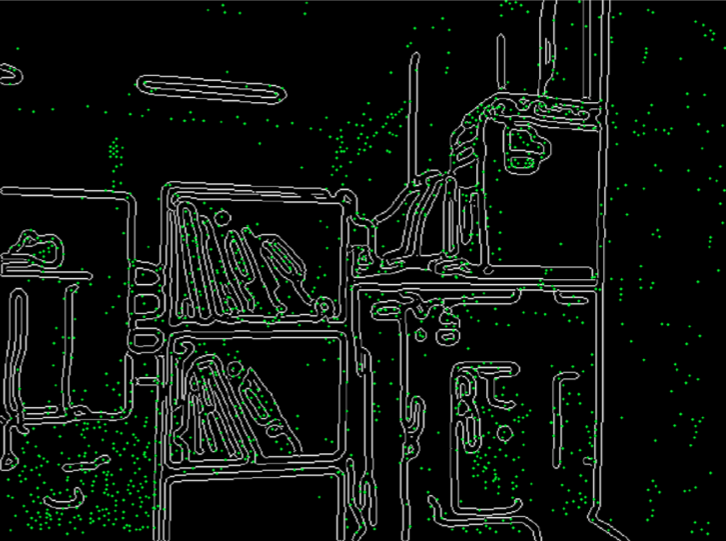
\includegraphics[resolution=150, scale=0.5]{images/lee-sift-mops-example}
  \caption{Example output for combined SIFT and MOPS features.}
  \label{fig:lee-sift-mops}
\end{figure*}

We now determine the ``type'' of the object, based on comparison of the distance of SIFT features within an outline to the distance to MOPS features on the outline. Define $D_M$ to be the distance to a MOPS feature, and $D_S$ to be the distance to a SIFT feature within the outline. Let $T_1$ and $T_2$ be two threshold values. We have the following equations
\begin{equation}
  \label{eq:dist1}
  | D_M - D_S | \leq T_1
\end{equation}
\begin{equation}
  \label{eq:dist2}
  T_1 < | D_M - D_S | \leq T_2
\end{equation}
\begin{equation}
  \label{eq:dist3}
  T_2 < | D_M - D_S |
\end{equation}

$T_1$ should be set such that there is a high probabilitiy that the SIFT and MOPS features are on the same object, and $T_2$ such that there is a high probability that the features are on different objects. We thus have the following cases:
\begin{itemize}
\item Equation~\ref{eq:dist1} is the case of an object with a closed interior.
\item Equation~\ref{eq:dist2} is again the case where an object has a closed interior, but possibly with a convex shape.
\item Equation~\ref{eq:dist3} is the case of an object with an open interior.
\end{itemize}
In the third case, we repeat the above process feature points on an object behind the open space.

This comparison allows us to determine what sort of obstacle an object is and to locate where in the world the objects exist, relative to the quadrotor.

\subsection{Replacing MOPS with Contours}
After finding object outlines using MOPS features to not give sufficient information, we sought an 
alternative approach.  As~\cite{suzuki1985} has been widely tested and locates contours within an image it appeared to be 
sufficient to locate the outlines of objects. We used the Canny Edge Detector~\cite{canny1986} to convert to binary images as the input to
this method.  After locating the contours in an image we marked the key points found using the SIFT algorithm as 
belonging to an object outline and proceeded as normal through the rest of the approach of~\cite{lee2011} (see Figure~\ref{fig:contour-ex}).

\subsection{Integrating PTAM}
Integrating PTAM with the quadrotor is remarkably simple. We made use of two different methods to accomplish this, in order to have different features available. Both methods rely upon the Robot Operating System (ROS)~\cite{ros} for support and the ardrone\_autonomy~\cite{ardroneautonomy} driver for communication with the quadrotor.

Our first approach is to directly test PTAM on data from the quadrotor. For this, we made use of the ethzasl\_ptam package~\cite{ethzaslptam}, which integrates PTAM with ROS. It was then only a matter of converting the camera stream from the ardrone\_autonomy driver to the requisite format for use with PTAM and calibrating the camera appropriately.

Secondly, we made use of the tum\_ardrone~\cite{tumardrone} package for ROS, which integrates a version of PTAM with an extended Kalman filter for data fusion and state estimation and a system for generating steering commands for the quadrotor. tum\_ardrone builds upon PTAM to provide an environment specifically designed for use with the ARDrone and ARDrone 2, and in addition to obstacle detection, provides a system for navigation and auto-pilot.

\section{Experiments}
Our data sets consist of samples obtained by recording output from the quadrotor's forward-facing camera. These are $640 \times 360$ pixel colour images saved in JPEG format recorded at a rate of one per each $0.01$ second. Our initial data sets consisted of
\begin{itemize}
\item A set of 212 frames in which the drone is sitting still on a table.
\item A set of 321 frames in which the drone takes off, flies down a Siebel Center hall, and lands.
\item A set of 301 frames in which the drone takes off, flies through the Siebel Center atrium, and lands.
\end{itemize}
These were supplemented with the following additional data sets from the quadrotor, this time recorded at a rate of one per each $0.1$ second.
\begin{itemize}
\item A set of 130 frames in which the drone flies through the Siebel Center atrium with additional movement, and people present.
\item A set of 275 frames in which the drone flies closely along the pillars and display cases of in the Siebel Center atrium.
\item A set of 49 frames in which the drone flies towards a corner in the Siebel Center atrium.
\end{itemize}

We additionally conducted experiments in which we evaluated methods on live data from the quadrotor while it was flying.

\subsection{Lee et al.}
We began by evaluating the SIFT and MOPS features on samples from our data sets. As this is the basis upon which the rest of the approach is built, this is a reasonable place to begin. SIFT keypoints and the computed matches for a sample image are shown in Figure~\ref{fig:sift-ex}. As can be seen, the matches between keypoints in general appear to be reasonable.

Figure~\ref{fig:mops-ex} displays results for MOPS keypoints and matches on the same frame pair as above. These are quite poor, and further discussion is made of this in the analysis section. Additionally, it was found that extraction of MOPS descriptors and matching took an much more time than would be appropriate for this application (several seconds) in any situation other than highly constrained thresholds to eliminate most points.

To validate that our feature point detection for MOPS was correct, we took several sample images from our data sets and ran the VLFeat~\cite{vlfeat} multi-scale Harris corner detector on the images. Results for one such image are displayed in Figure~\ref{fig:vlfeat-ex}. It should be noted that the detected keypoints in that image are quite similar to those detected in the MOPS sample images; as is expected, since MOPS makes use of a multi-scale Harris corner detector.

\subsection{Contours}
Subsequently we replaced MOPS features with contours on which we detected SIFT keypoints; see Figure~\ref{fig:contour-ex} for example results, again on the same frame pair. While these results are better than with MOPS, they again are insufficient.

\subsection{PTAM}
PTAM was evaluated on a live-stream from the quadrotor as it flew, as it could not be meaningfully evaluated on the sample data sets we had recorded. PTAM was able to successfully initialize and maintain a map of its environment which included the relative distance from the quadrotor to objects. An example map of the environment produced by PTAM is shown in Figure~\ref{fig:ptam-ex}.

This performance was sufficient for real-time operation, and we were able to successfully fly the quadrotor through environments using the tum\_ardrone package.  See our supplementary video to observe PTAM's performance during one of our test flights.

\begin{figure*}[h]
  \centering
  \begin{tabular}{cc}
    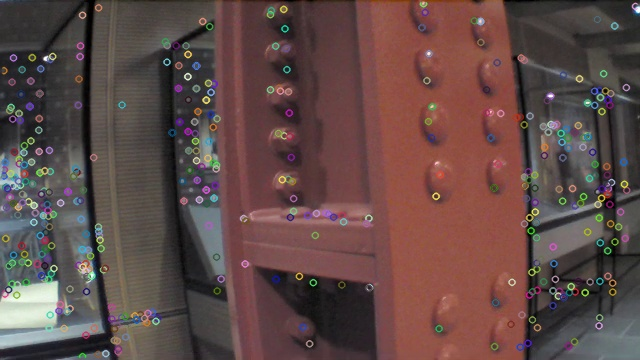
\includegraphics[resolution=150, scale=0.75]{images/sift-kp1} &
    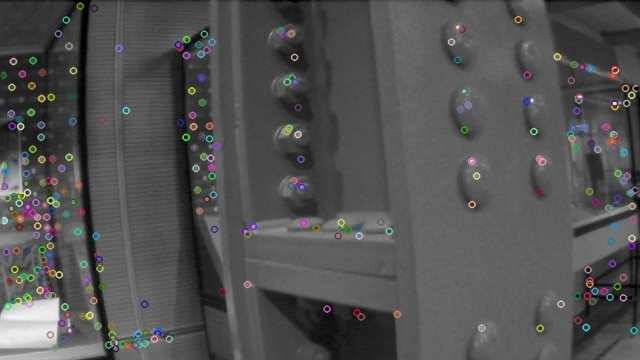
\includegraphics[resolution=150, scale=0.75]{images/sift-kp2} \\
    \multicolumn{2}{c}{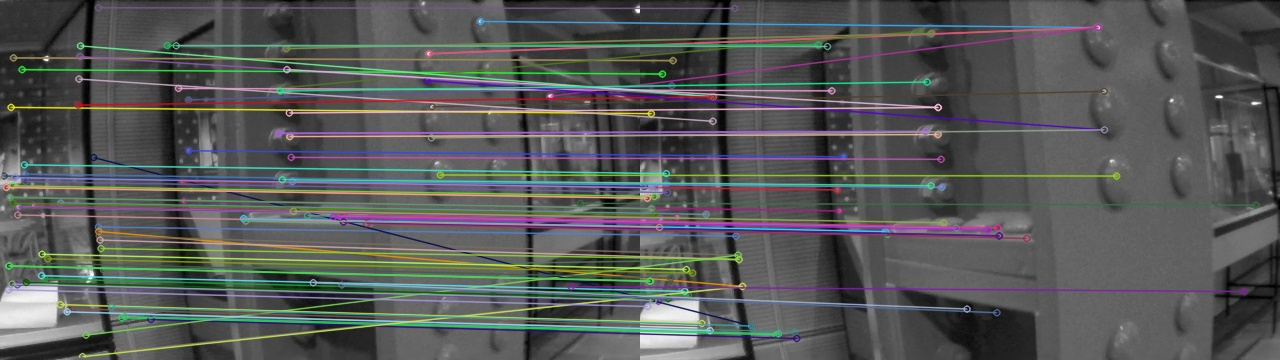
\includegraphics[resolution=150, scale=0.77]{images/sift-matches}}
  \end{tabular}
  \caption{SIFT keypoints and matches.}
  \label{fig:sift-ex}
\end{figure*}

\begin{figure*}[h]
  \centering
  \begin{tabular}{cc}
    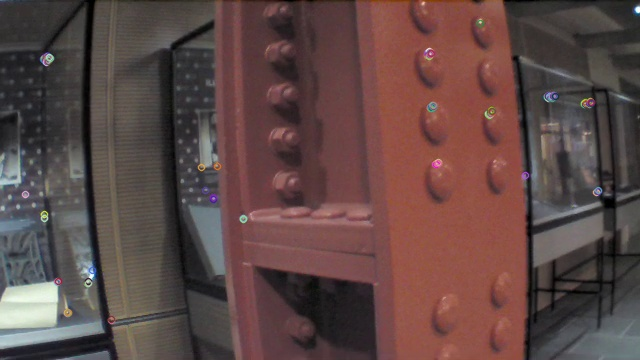
\includegraphics[resolution=150, scale=0.75]{images/mops-kp1} &
    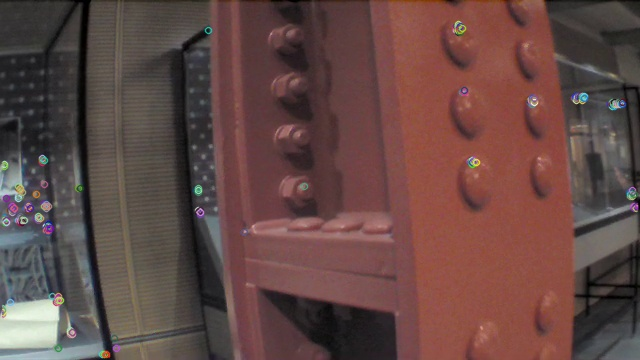
\includegraphics[resolution=150, scale=0.75]{images/mops-kp2} \\
    \multicolumn{2}{c}{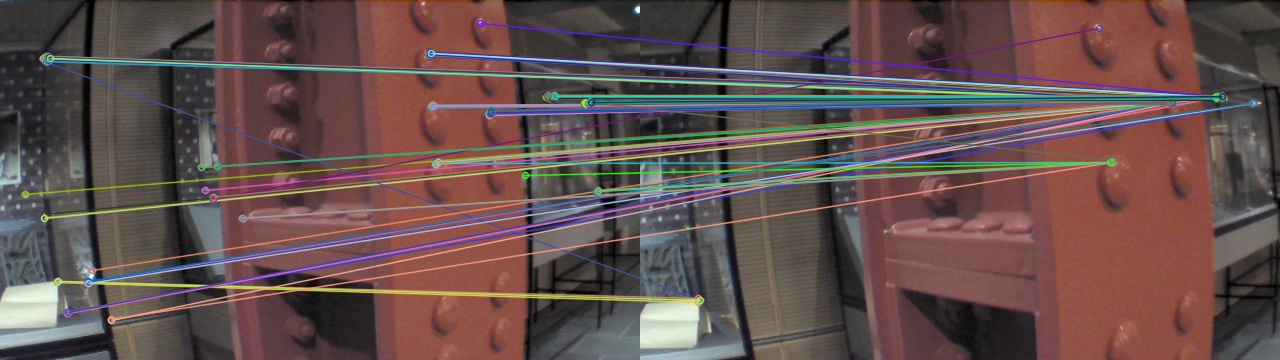
\includegraphics[resolution=150, scale=0.77]{images/mops-matches}}
  \end{tabular}
  \caption{MOPS keypoints and matches.}
  \label{fig:mops-ex}
\end{figure*}

\begin{figure*}[h]
  \centering
  \begin{tabular}{cc}
    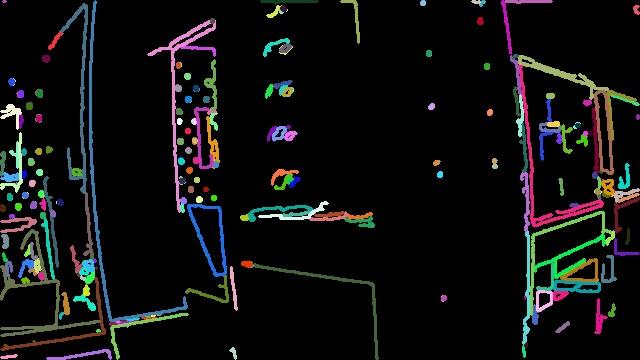
\includegraphics[resolution=150, scale=0.75]{images/contour-lines1} &
    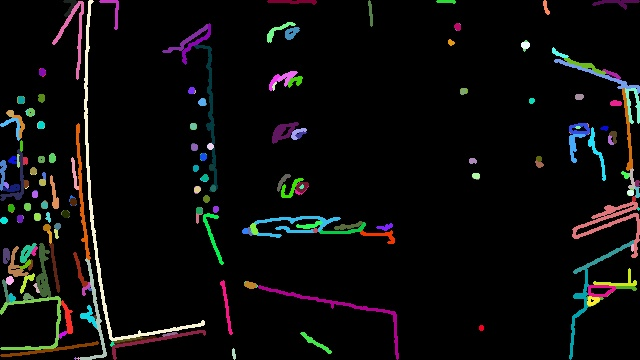
\includegraphics[resolution=150, scale=0.75]{images/contour-lines2} \\
    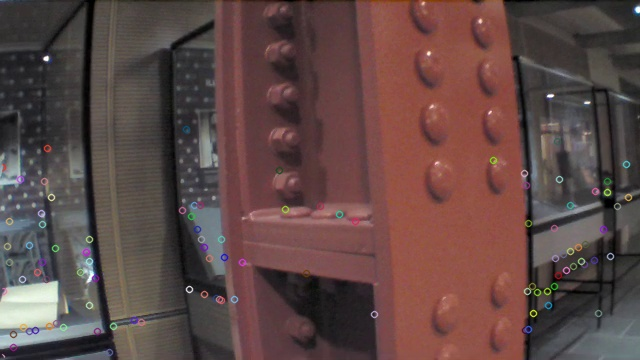
\includegraphics[resolution=150, scale=0.75]{images/contour-kp1} &
    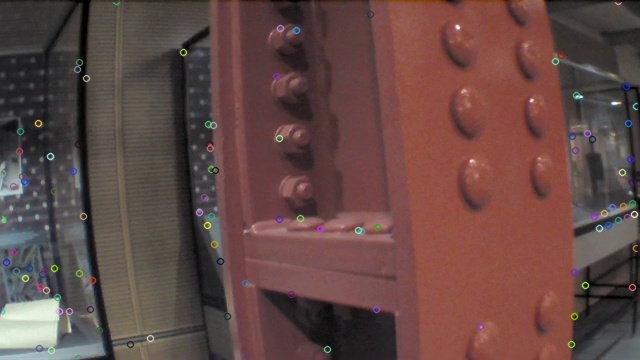
\includegraphics[resolution=150, scale=0.75]{images/contour-kp2} \\
    \multicolumn{2}{c}{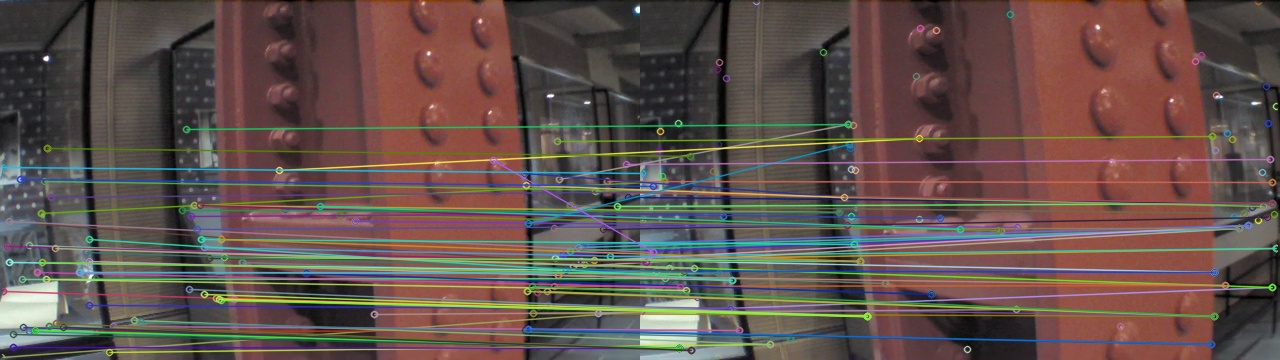
\includegraphics[resolution=150, scale=0.77]{images/contour-matches}}
  \end{tabular}
  \caption{Contour lines, keypoints, and matches.}
  \label{fig:contour-ex}
\end{figure*}

\begin{figure*}[h]
  \centering
  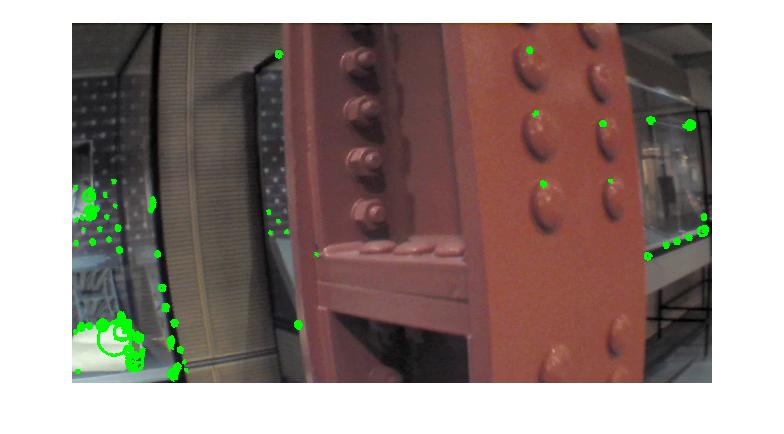
\includegraphics[resolution=150, scale=0.75]{images/vlfeat-kp2}
  \caption{VLFeat multi-scale Harris corner detector keypoints.}
  \label{fig:vlfeat-ex}
\end{figure*}

\begin{figure*}[h]
  \centering
  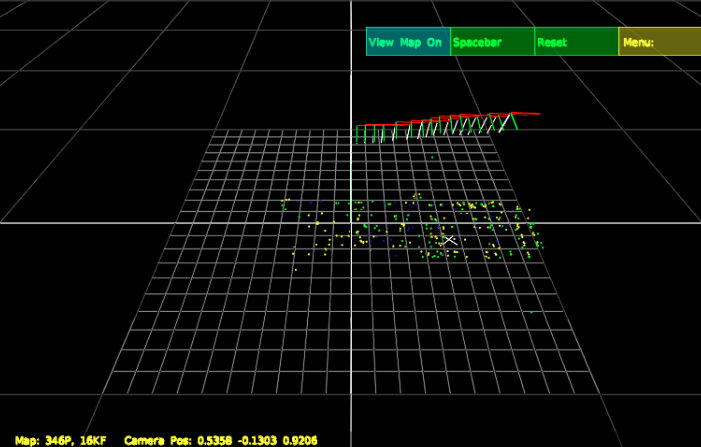
\includegraphics[resolution=150, scale=0.5]{images/ptam-map}
  \caption{PTAM-generated environment map.}
  \label{fig:ptam-ex}
\end{figure*}

\section{Analysis}
During our experiments we considered the following factors as the primary characteristics the algorithm must possess in order
to be be appropriate for our task:

\begin{enumerate}
 \item It must robustly produce an accurate 3D model of the world.
 \item It must run in real time.
\end{enumerate}

If an algorithm is unable to create an accurate representation of a scene then it would be unsuitable to use for navigation
purposes.  On the other hand, if it is unable to run in real time collision information may not be available until it is too
late to avoid the obstacle.  Both factors were considered equally important in our evaluation.

As~\cite{lee2011} proposed to use a sparse representation in the pursuit of real time performance, one of our primary 
concerns was if the 3D model it creates would be suitable for our task.  Upon inspecting the results of the tests described
in Section 4.1, it was obvious that the matches were very noisy, and the subsequent reconstruction using the punitive matches
did not produce a model that was representative of the scene.  Of particular note in the case of the example shown was the 
few number of features detected along the pillar.  The lack of many MOPS features on the pillar indicates 
that our object outlines would not be very representative of its true location, making autonomous navigation risky.  While 
this by itself intensified the misgivings on the approach, it was not clear that an alternative to the MOPS features could 
not produce a better representation as the SIFT features did provide better punitive matches.

This was reinforced with our test using image contours rather than MOPS features as we were able to create a better set of
punitive matches between the images.  While the reconstruction using these matches still produced a 3D model that would not
be sufficient for our task, it does indicate that additional work could be performed in this space that would see better
results.  In addition, it is important to note that while the display cases in the presented example present additional
challenges for any reconstruction effort, the algorithm did not produce good results in images without any glass in the 
frame.  

Even though some progress was made to create a more accurate representation, it came at the cost of increasing the
number of features in a scene and the computational effort that would be necessary for navigation.  Since we focus on 
reducing the number of keypoints used for matching and reconstruction, it also amplifies the effect poor matches have on
our algorithm making it sensitive to noise.  From this analysis it follows that if we were able to compute a large number of
features very quickly, even if we had several bad matches they would have less effect on our solution.

Using this line of reasoning we explored the effectiveness of the PTAM approach.  This algorithm has been demonstrated to
perform at 20Hz on a computationally limited platform (an ATOM 1.6GHz single core processor) using up to 300 keypoints in each
image to create the punitive matches with a RMS error in its position of 3.02cm or less along any axis~\cite{weiss2011}. This
approach is not without its own drawbacks, however.

In~\cite{weiss2011} they recommend at least 90 percent overlap between frames for good tracking. In our own test flights 
using this system we found that the quadrotor's position was lost in the map when stopping suddenly, and rotations also 
contributed to position errors and should be avoided as much as possible.  As with many other vision based applications, 
textureless surfaces continue to be a problem and can result in loss of a quadrotor's position.  This seems to point to using 
a downward facing camera to avoid rotations. This would help increase the probability of obtaining a feature rich map by 
using a wide field of view camera as a way of reducing the impact of these restrictions.

\section{Individual Contributions}
Individual contributions break down roughly as follows. Nikoli was responsible for:
\begin{itemize}
\item Implementing SIFT feature detection, extraction, and image matching
\item Implementing 3-D reconstruction and triangulation
\item Implementing the multi-threaded image pipeline
\item Setting up and integrating ethzasl\_ptam with the quadrotor
\item Setting up tum\_ardrone
\item Experimental evaluations
\item Presentation and paper writing
\end{itemize}

Bryan was responsible for:
\begin{itemize}
\item Implementing MOPS feature detection, extraction, and image matching
\item Experimenting with a contour-based technique to replace MOPS
\item Assistance with 3-D reconstruction
\item Assistance with setting up ethzasl\_ptam
\item Experimental evaluations
\item Presentation and paper writing
\end{itemize}

Because MOPS was implemented from scratch, we feel that the work was split quite evenly.

\bibliographystyle{acmsiggraph}
\bibliography{bib_all}
\end{document}


